% !Mode:: "TeX:UTF-8"
\documentclass[leqno]{article}
\input{en_preamble.tex}
\input{xecjk_preamble.tex}
\setCJKmainfont{STKaiti} % 如果请替换为本地系统有的字体
%中文断行
\XeTeXlinebreaklocale "zh"
\XeTeXlinebreakskip = 0pt plus 1pt minus 0.1pt
\usetikzlibrary{decorations,arrows}
\usetikzlibrary{decorations.markings}
\makeatletter % `@' now normal "letter"
\@addtoreset{equation}{section}
\makeatother  % `@' is restored as "non-letter"
\renewcommand\theequation{\oldstylenums{\thesection}%
                   .\oldstylenums{\arabic{equation}}}
\begin{document}
\title{Darcy-forchheimer Equation的块中心差分方法(二维)}
\author{李奥}
\date{\today}
\maketitle
\tableofcontents
\newpage
\section{符号}
\begin{tabular}{ |l|l| }   
\hline   
\multicolumn{2}{|c|}{符号说明} \\  
\hline
符号 & 意义 \\
\hline
$\Omega$ & $(0,1)\times(0,1)$(二维区域) \\
\hline
$p$ & 压强(压力) \\
\hline
$\boldsymbol{u}$ & 流体速度 \\
\hline
$\mu$ & 黏性系数 \\
\hline
$K$ & 渗透张量 \\
\hline
$k$ & 正数且 K = kI(I 是单位矩阵) \\
\hline 
$\beta$ & 非线性项系数 \\
\hline
$\rho$ & 流体密度 \\
\hline
$\boldsymbol{f}$ & $\boldsymbol{f} \in (L(\Omega)^2)^2$, a vector function\\
\hline
$g(\boldsymbol{x})$ & $g(\boldsymbol{x}) \in L^2(\Omega)$, a scalar function \\
\hline 
$nx$ & $x$ 方向剖分的段数 \\
\hline
$ny$ & $y$ 方向剖分的段数 \\
\hline
$h_x$ & $x$ 方向剖分的步长 \\
\hline
$h_y$ & $y$ 方向剖分的步长 \\
\hline
$NC$ & 单元个数 \\
\hline
$NE$ & 边的个数 \\
\hline
\end{tabular}

\section{模型}
\begin{equation*}
\begin{cases}
\begin{aligned}
(\frac{\mu}{k} + \beta\rho|\boldsymbol{u}|)\boldsymbol{u} + \nabla p & = \boldsymbol{f} \quad in \,\ \Omega = (0,1)\times (0,1) \\
\nabla \cdot \boldsymbol{u} & = g \quad in \,\ \Omega \\
\boldsymbol {u} & = 0 \quad on \,\ \partial \Omega
\end{aligned}
\end{cases}
\end{equation*}


记$\boldsymbol{u} = \dbinom{u}{v}$,那么有\\

\begin{equation*}
\begin{cases}
\begin{aligned}
(\frac{\mu}{k} + \beta\rho|\boldsymbol{u}|)u + \nabla_x p & = f_1 \quad (i) \\
(\frac{\mu}{k} + \beta\rho|\boldsymbol{u}|)v + \nabla_y p & = f_2 \quad (ii) \\
\partial_x u + \partial_y v & = g \quad (iii)
\end{aligned}
\end{cases}
\end{equation*}

\section{差分离散}

利用一阶向前差分把方程变成差分方程,现在从 $cell$ 和 $edge$ 的角度考虑模型。\\
对于 $(i)$,从内部纵向 $edge$ 的角度考虑:我们需要找到内部纵向 $edge$ 所对应的左手边的 $cell$ 和右手边的 $cell$. 左右两边的$cell$ 所对应的 $p$ 分别记为 $p_{l}$、$p_{r}$.$u$ 为 $edge$ 的$y$ 方向的 $m$ 条边中点,记为 $u_m$。按照 $mesh$ 里的编号规则排序。\\

则每条内部边上所对应的差分方程为:

\begin{equation}\label{eq:um}
(\frac{\mu}{k} + \beta\rho\left|\boldsymbol{u}\right|) \cdot u_m + \frac{p_r - p_l}{h^x_{i+1/2}} = f_{1,m}
\end{equation}

\begin{figure}[H] 
\centering 
\includegraphics[scale=0.6]{edge_y.png} 
\caption{$edge_y$} 
\label{fig:label} 
\end{figure}

对于 $(ii)$,从内部横向 $edge$ 的角度考虑:
我们需要找到内部横向 $edge$ 所对应的左手边的 $cell$ 和右手边的 $cell$. $cell$ 所对应的 $p$ 与 $(i)$ 中的相同。$v$ 为 $edge$ 的$x$ 方向的 $m$ 个中点,记为 $v_m$。\\

则每条内部边上所对应的差分方程为:\\

\begin{equation}\label{eq:vm}
(\frac{\mu}{k} + \beta\rho\left|\boldsymbol{u}\right|) \cdot v_m + \frac{p_l - p_r}{h^y_{j+1/2}} = f_{2,m}
\end{equation}

\begin{figure}[H] 
\centering 
\includegraphics[scale=0.6]{edge_x.png} 
\caption{$edge_x$} 
\label{fig:label} 
\end{figure}

对于 $(iii)$, 从 $cell$ 的角度考虑:
由于单元是四边形单元,我们记单元所对应边的局部编号为[0,1,2,3](StructureQuadMesh.py 里的网格),第 $i$ 个单元所对应的边记为 $e_{i,0},e_{i,1},e_{i,2},e_{i,3}$。\\

则 $(iii)$ 式第 $i$ 个单元所对应的差分方程为:\\

\begin{equation}\label{eq:uv}
\frac{u_{e_{i,1}} - u_{e_{i,3}}}{h^x_i} + \frac{v_{e_{i,2}} - v_{e_{i,0}}}{h^y_i} = g_i
\end{equation}

\begin{figure}[H] 
\centering 
\includegraphics[scale=0.6]{cell.png} 
\caption{cell} 
\label{fig:label} 
\end{figure}

现在我们先求解 $p$, 再求解 $\boldsymbol{u}$.\\

对于 $\eqref{eq:um}$ 我们有

\begin{equation}\label{eq:up}
u_m = \frac{f_{1,m} - \frac{p_{r} - p_{l}}{h^x_{i+1/2}}}{(\mu/k+\beta\rho\left|\boldsymbol{u}\right|)_m} 
\end{equation}

对于 $\eqref{eq:vm}$ 我们有
\begin{equation}\label{eq:vp}
v_m = \frac{f_{2,m} - \frac{p_{a} - p_{d}}{h^y_{j+1/2}}}{(\mu/k+\beta\rho\left|\boldsymbol{u}\right|)_m} 
\end{equation}

注: 记$\mu/k+\beta\rho\left|\boldsymbol{u}\right| = C$,  $p_{l,1}$ 、$p_{r,3}$ 、$p_{a,0}$ 和 $p_{d,2}$ 是同一个点处的 $p$, 记为$p_i$.

且有
\begin{equation*}
\begin{aligned}
\frac{f_{1,1} - \frac{p_{r,1} - p_{l,1}}{h^x_i}}{C_{i,1}} & = \mathcal{W}_{i,1} \\
\frac{f_{1,3} - \frac{p_{r,3} - p_{l,3}}{h^x_i}}{C_{i,3}} & = \mathcal{W}_{i,3} \\
\frac{f_{2,2} - \frac{p_{a,2} - p_{d,2}}{h^y_i}}{C_{i,2}} & = \mathcal{W}_{i,2} \\
\frac{f_{2,0} - \frac{p_{a,0} - p_{d,0}}{h^y_i}}{C_{i,0}} & = \mathcal{W}_{i,0}
\end{aligned}
\end{equation*}\\

\begin{equation*}
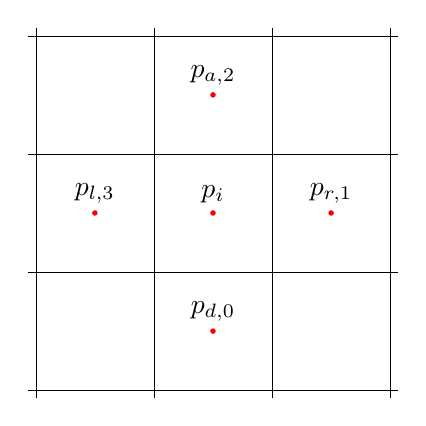
\begin{tikzpicture}
\draw[very thin,color=black,step=1.5cm](-0.1,-0.1) grid (4.6,4.6);
\fill[red] (2.25,0.75) circle [radius=1pt];
\fill[red] (0.75,2.25) circle [radius=1pt];
\fill[red] (2.25,2.25) circle [radius=1pt];
\fill[red] (3.75,2.25) circle [radius=1pt];
\fill[red] (2.25,3.75) circle [radius=1pt];

\node[above] at (2.25,0.75){$p_{d,0}$};
\node[above] at (0.75,2.25){$p_{l,3}$};
\node[above] at (2.25,2.25){$p_{i}$};
\node[above] at (3.75,2.25){$p_{r,1}$};
\node[above] at (2.25,3.75){$p_{a,2}$};
\end{tikzpicture}
\end{equation*}
\subsection{均匀剖分}
由于这里的方法是均匀剖分,所以离散形式中的 $x,y$ 方向的步长可以用 $h_x,h_y$ 统一表示。
\subsubsection{求解$p$的显式格式}

要求解 $p$,我们把 $\eqref{eq:up}$ 和 $\eqref{eq:vp}$ 代入到 $\eqref{eq:uv}$ 即可。但是,我们现在需要分情况讨论: \\

1).当$u_{i,3}$ 与 $v_{i,0}$ 是边界边上中点的值时(左下角的边界函数),有

\begin{equation*}
\frac{\mathcal{W}_{i,1} - u_{i,3}}{h_x} + \frac{\mathcal{W}_{i,2} - v_{i,0}}{h_y} = g_i
\end{equation*} 

整理后得到:

\begin{equation*}
(\frac{1}{h_x^2C_{i,1}} + \frac{1}{h_y^2C_{i,2}})p_i = g_i - \frac{h_xf_{1,1}}{h_x^2C_{i,1}} - \frac{h_yf_{1,2}}{h_y^2C_{i,2}} + \frac{p_{r,1}}{h_x^2C_{i,1}} + \frac{p_{a,2}}{h_y^2C_{i,2}} + \frac{u_{i,3}}{h_x} + \frac{v_{i,0}}{h_y}
\end{equation*}

2).当$u_{e_{i,3}}$ 与 $v_{e_{i,2}}$ 是边界边上中点的值时(左上角的边界单元),有

\begin{equation*}
\frac{\mathcal{W}_{e_{i,1}} - u_{e_{i,3}}}{h_x} + \frac{ v_{e_{i,2}} - \mathcal{W}_{e_{i,0}}}{h_y} = g_i
\end{equation*} 

整理后得到:

\begin{equation*}
(\frac{1}{h_x^2C_{i,1}} + \frac{1}{h_y^2C_{i,0}})p_i = g_i - \frac{h_xf_{1,1}}{h_x^2C_{i,1}} + \frac{h_yf_{1,0}}{h_y^2C_{i,0}} + \frac{p_{r,1}}{h_x^2C_{i,1}} + \frac{p_{d,0}}{h_y^2C_{i,0}} + \frac{u_{i,3}}{h_x} - \frac{v_{i,2}}{h_y}
\end{equation*}

3).当$u_{i,1}$ 与 $v_{i,0}$ 是边界边上中点的值时(右下角的边界单元),有

\begin{equation*}
\frac{ u_{i,1} - \mathcal{W}_{i,3}}{h_x} + \frac{\mathcal{W}_{i,2} - v_{i,0}}{h_y} = g_i
\end{equation*} 

整理后得到:

\begin{equation*}
(\frac{1}{h_x^2C_{i,3}} + \frac{1}{h_y^2C_{i,2}})p_i = g_i + \frac{h_xf_{1,3}}{h_x^2C_{i,3}} - \frac{h_yf_{1,2}}{h_y^2C_{i,2}} + \frac{p_{l,3}}{h_x^2C_{i,3}} + \frac{p_{a,2}}{h_y^2C_{i,2}} - \frac{u_{i,1}}{h_x} + \frac{v_{i,0}}{h_y}
\end{equation*}

4).当$u_{i,1}$ 与 $v_{i,2}$ 是边界边上中点的值时(右上角的边界单元),有

\begin{equation*}
\frac{ u_{i,1} - \mathcal{W}_{i,3}}{h_x} + \frac{ v_{i,2} - \mathcal{W}_{i,0}}{h_y} = g_i
\end{equation*} 

整理后得到:

\begin{equation*}
(\frac{1}{h_x^2C_{i,3}} + \frac{1}{h_y^2C_{i,0}})p_i = g_i + \frac{h_xf_{1,3}}{h_x^2C_{i,3}} + \frac{h_yf_{1,0}}{h_y^2C_{i,0}} + \frac{p_{l,3}}{h_x^2C_{i,3}} + \frac{p_{d,0}}{h_y^2C_{i,0}} - \frac{u_{i,1}}{h_x} - \frac{v_{i,2}}{h_y}
\end{equation*}

5).当$u_{i,3}$ 是边界边上的中点的值时(左边的边界单元),有

\begin{equation*}
\frac{\mathcal{W}_{i,1} - u_{i,3}}{h_x} + \frac{\mathcal{W}_{i,2} - \mathcal{W}_{i,0}}{h_y} = g_i
\end{equation*}

整理后得到:

\begin{equation*}
\begin{aligned}
(\frac{1}{h_x^2C_{i,1}} + \frac{1}{h_y^2C_{i,0}} + \frac{1}{h_y^2C_{i,2}})p_i = & g_i - \frac{h_xf_{1,1}}{h_x^2C_{i,1}} - \frac{h_yf_{1,2}}{h_y^2C_{i,2}} + \frac{h_yf_{1,0}}{h_y^2C_{i,0}}\\
& + \frac{p_{r,1}}{h_x^2C_{i,1}} + \frac{p_{d,0}}{h_y^2C_{i,0}} + \frac{p_{a,2}}{h_y^2C_{i,2}} + \frac{u_{i,3}}{h_x}
\end{aligned}
\end{equation*}

6).当$u_{i,1}$ 是边界边上中点的值时(右边的边界单元),有
\begin{equation*}
\frac{ u_{i,1} - \mathcal{W}_{i,3}}{h_x} + \frac{ \mathcal{W}_{i,2} - \mathcal{W}_{i,0}}{h_y} = g_i
\end{equation*} 

整理后得到:

\begin{equation*}
\begin{aligned}
(\frac{1}{h_x^2C_{i,1}} + \frac{1}{h_y^2C_{i,0}} + \frac{1}{h_y^2C_{i,2}})p_i = & g_i + \frac{h_xf_{1,3}}{h_x^2C_{i,3}} - \frac{h_yf_{1,2}}{h_y^2C_{i,2}} + \frac{h_yf_{1,0}}{h_y^2C_{i,0}}\\
& + \frac{p_{l,3}}{h_x^2C_{i,1}} + \frac{p_{d,0}}{h_y^2C_{i,0}} + \frac{p_{a,2}}{h_y^2C_{i,2}} - \frac{u_{i,1}}{h_x}
\end{aligned}
\end{equation*}

7).当$v_{i,0}$ 是边界边上中点的值时(下边的边界单元),有

\begin{equation*}
\frac{ \mathcal{W}_{i,1} - \mathcal{W}_{i,3}}{h_x} + \frac{\mathcal{W}_{i,2}- v_{i,0}}{h_y} = g_i
\end{equation*} 

整理后得到:

\begin{equation*}
\begin{aligned}
(\frac{1}{h_x^2C_{i,1}} + \frac{1}{h_x^2C_{i,3}} + \frac{1}{h_y^2C_{i,2}})p_i =& g_i - \frac{h_xf_{1,1}}{h_x^2C_{i,1}} + \frac{h_xf_{1,3}}{h_x^2C_{i,3}} - \frac{h_yf_{1,2}}{h_y^2C_{i,2}}\\
& + \frac{p_{r,1}}{h_x^2C_{i,1}} + \frac{p_{l,3}}{h_x^2C_{i,3}} + \frac{p_{a,2}}{h_y^2C_{i,2}} + \frac{v_{i,0}}{h_y}
\end{aligned}
\end{equation*}

8).当$v_{i,2}$ 是边界边上中点的值时(上边的边界单元),有

\begin{equation*}
\frac{ \mathcal{W}_{i,1} - \mathcal{W}_{i,3}}{h_x} + \frac{ v_{i,2} - \mathcal{W}_{i,0}}{h_y} = g_i
\end{equation*} 

整理后得到:

\begin{equation*}
\begin{aligned}
(\frac{1}{h_x^2C_{i,1}} + \frac{1}{h_x^2C_{i,3}} + \frac{1}{h_y^2C_{i,0}})p_i =& g_i - \frac{h_xf_{1,1}}{h_x^2C_{i,1}} + \frac{h_xf_{1,3}}{h_x^2C_{i,3}} + \frac{h_yf_{1,0}}{h_y^2C_{i,0}}\\
& + \frac{p_{r,1}}{h_x^2C_{i,1}} + \frac{p_{l,3}}{h_x^2C_{i,3}} + \frac{p_{d,0}}{h_y^2C_{i,0}} - \frac{v_{i,2}}{h_y}
\end{aligned}
\end{equation*}

9).全部为内部边的中点的值时(内部单元),有

\begin{equation*}
\frac{ \mathcal{W}_{i,1} - \mathcal{W}_{i,3}}{h_x} + \frac{ \mathcal{W}_{i,2} - \mathcal{W}_{i,0}}{h_y} = g_i
\end{equation*} 

整理后得到:

\begin{equation*}
\begin{aligned}
(\frac{1}{h_x^2C_{i,1}} + \frac{1}{h_x^2C_{i,3}} + \frac{1}{h_y^2C_{i,0}} + \frac{1}{h_y^2C_{i,2}})p_i =& g_i - \frac{h_xf_{1,1}}{h_x^2C_{i,1}} + \frac{h_xf_{1,3}}{h_x^2C_{i,3}} - \frac{h_yf_{1,2}}{h_y^2C_{i,2}} + \frac{h_yf_{1,0}}{h_y^2C_{i,0}}\\
& + \frac{p_{r,1}}{h_x^2C_{i,1}} + \frac{p_{l,3}}{h_x^2C_{i,3}} + \frac{p_{d,0}}{h_y^2C_{i,0}} + \frac{p_{a,2}}{h_y^2C_{i,2}}
\end{aligned}
\end{equation*}

对于边界单元的 $p$,需要做下特殊处理:\\

1) $u$ 的左边的单元与 $u$ 本身相等时

\begin{equation*}
\begin{aligned}
C_{\frac{1}{2}}u_{\frac{1}{2}} + \nabla p & = f_{1,\frac{1}{2}}\\
\Rightarrow \frac{p_l - p_r}{h_x} & = f_{1,\frac{1}{2}} - C_{\frac{1}{2}}u_{\frac{1}{2}} \\
\Rightarrow p_r & = - h_xf_{1,\frac{1}{2}} + h_xC_{\frac{1}{2}}u_{\frac{1}{2}} + p_l
\end{aligned}
\end{equation*} 

2) $u$ 的右边的单元与 $u$ 本身相等时

\begin{equation*}
\begin{aligned}
C_{Nx+\frac{1}{2}}u_{Nx+\frac{1}{2}} + \nabla p & = f_{1,Nx+\frac{1}{2}}\\
\Rightarrow \frac{p_r - p_l}{h_x} & = f_{1,Nx+\frac{1}{2}} - C_{Nx+\frac{1}{2}}u_{Nx+\frac{1}{2}} \\
\Rightarrow p_r & =  h_xf_{1,\frac{1}{2}} - h_xC_{\frac{1}{2}}u_{\frac{1}{2}} + p_l
\end{aligned}
\end{equation*} 

3) $v$ 的下边的单元与 $v$ 本身相等时

\begin{equation*}
\begin{aligned}
C_{\frac{1}{2}}v_{\frac{1}{2}} + \nabla p & = f_{2,\frac{1}{2}}\\
\Rightarrow \frac{p_l - p_r}{h_y} & = f_{2,\frac{1}{2}} - C_{\frac{1}{2}}v_{\frac{1}{2}} \\
\Rightarrow p_r & = - h_yf_{2,\frac{1}{2}} + h_yC_{\frac{1}{2}}v_{\frac{1}{2}} + p_l
\end{aligned}
\end{equation*} 

4) $v$ 的上边的单元与 $v$ 本身相等时

\begin{equation*}
\begin{aligned}
C_{Ny+\frac{1}{2}}v_{Ny+\frac{1}{2}} + \nabla p & = f_{2,Ny+\frac{1}{2}}\\
\Rightarrow \frac{p_r - p_l}{h_y} & = f_{2,Ny+\frac{1}{2}} - C_{Ny+\frac{1}{2}}v_{Ny+\frac{1}{2}} \\
\Rightarrow p_r & = h_yf_{2,Ny+\frac{1}{2}} - h_yC_{Ny+\frac{1}{2}}v_{Ny+\frac{1}{2}} + p_l
\end{aligned}
\end{equation*}

\begin{figure}[H] 
\centering 
\includegraphics[scale=0.6]{mesh.png} 
\caption{$mesh$} 
\label{fig:label} 
\end{figure}

再求解$\boldsymbol{u}$:
\begin{equation*}
\begin{aligned}
u_m & = (f_{1,m} - \frac{p_{r} - p_{l}}{h_x})/C_m \\
v_m & = (f_{2,m} - \frac{p_{l} - p_{r}}{h_y})/C_m
\end{aligned}
\end{equation*}
\subsubsection{求解 $p$ 的隐格式}

与上面一部分一样,我们先求解 $p$, 再求解 $\boldsymbol{u}$.\\
我们考虑 $C$ 的求解方法,在边界的时候,记$f = f_b$, 边界处的 $u,v$ 统一记为 $U$,则有

\begin{equation*}
f_b = CU
\end{equation*}

要求解 $p$,我们把 $\eqref{eq:up}$ 和 $\eqref{eq:vp}$ 代入到 $\eqref{eq:uv}$即可。但是,我们现在需要分情况讨论: \\

1).当$u_{i,3}$ 与 $v_{i,0}$ 是边界边上中点的值时(左下角的边界函数),有

\begin{equation*}
\frac{\mathcal{W}_{i,1} - u_{i,3}}{h_x} + \frac{\mathcal{W}_{i,2} - v_{i,0}}{h_y} = g_i
\end{equation*} 

整理后得到:

\begin{equation*}
(\frac{1}{h_x^2C_{i,1}} + \frac{1}{h_y^2C_{i,2}})p_i - \frac{p_{r,1}}{h_x^2C_{i,1}} - \frac{p_{a,2}}{h_y^2C_{i,2}} = g_i - \frac{h_xf_{1,1}}{h_x^2C_{i,1}} - \frac{h_yf_{1,2}}{h_y^2C_{i,2}} + \frac{u_{i,3}}{h_x} + \frac{v_{i,0}}{h_y}
\end{equation*}

2).当$u_{e_{i,3}}$ 与 $v_{e_{i,2}}$ 是边界边上中点的值时(左上角的边界单元),有

\begin{equation*}
\frac{\mathcal{W}_{e_{i,1}} - u_{e_{i,3}}}{h_x} + \frac{ v_{e_{i,2}} - \mathcal{W}_{e_{i,0}}}{h_y} = g_i
\end{equation*} 

整理后得到:

\begin{equation*}
(\frac{1}{h_x^2C_{i,1}} + \frac{1}{h_y^2C_{i,0}})p_i - \frac{p_{r,1}}{h_x^2C_{i,1}} - \frac{p_{d,0}}{h_y^2C_{i,0}} = g_i - \frac{h_xf_{1,1}}{h_x^2C_{i,1}} + \frac{h_yf_{1,0}}{h_y^2C_{i,0}} + \frac{u_{i,3}}{h_x} - \frac{v_{i,2}}{h_y}
\end{equation*}

3).当$u_{i,1}$ 与 $v_{i,0}$ 是边界边上中点的值时(右下角的边界单元),有

\begin{equation*}
\frac{ u_{i,1} - \mathcal{W}_{i,3}}{h_x} + \frac{\mathcal{W}_{i,2} - v_{i,0}}{h_y} = g_i
\end{equation*} 

整理后得到:

\begin{equation*}
(\frac{1}{h_x^2C_{i,3}} + \frac{1}{h_y^2C_{i,2}})p_i - \frac{p_{l,3}}{h_x^2C_{i,3}} - \frac{p_{a,2}}{h_y^2C_{i,2}} = g_i + \frac{h_xf_{1,3}}{h_x^2C_{i,3}} - \frac{h_yf_{1,2}}{h_y^2C_{i,2}} - \frac{u_{i,1}}{h_x} + \frac{v_{i,0}}{h_y}
\end{equation*}

4).当$u_{i,1}$ 与 $v_{i,2}$ 是边界边上中点的值时(右上角的边界单元),有

\begin{equation*}
\frac{ u_{i,1} - \mathcal{W}_{i,3}}{h_x} + \frac{ v_{i,2} - \mathcal{W}_{i,0}}{h_y} = g_i
\end{equation*} 

整理后得到:

\begin{equation*}
(\frac{1}{h_x^2C_{i,3}} + \frac{1}{h_y^2C_{i,0}})p_i - \frac{p_{l,3}}{h_x^2C_{i,3}} - \frac{p_{d,0}}{h_y^2C_{i,0}} = g_i + \frac{h_xf_{1,3}}{h_x^2C_{i,3}} + \frac{h_yf_{1,0}}{h_y^2C_{i,0}} - \frac{u_{i,1}}{h_x} - \frac{v_{i,2}}{h_y}
\end{equation*}

5).当$u_{i,3}$ 是边界边上的中点的值时(左边的边界单元),有

\begin{equation*}
\frac{\mathcal{W}_{i,1} - u_{i,3}}{h_x} + \frac{\mathcal{W}_{i,2} - \mathcal{W}_{i,0}}{h_y} = g_i
\end{equation*}

整理后得到:

\begin{equation*}
\begin{aligned}
(\frac{1}{h_x^2C_{i,1}} + \frac{1}{h_y^2C_{i,0}} + \frac{1}{h_y^2C_{i,2}})p_i & - \frac{p_{r,1}}{h_x^2C_{i,1}} - \frac{p_{d,0}}{h_y^2C_{i,0}} - \frac{p_{a,2}}{h_y^2C_{i,2}} \\
& = g_i - \frac{h_xf_{1,1}}{h_x^2C_{i,1}} - \frac{h_yf_{1,2}}{h_y^2C_{i,2}} + \frac{h_yf_{1,0}}{h_y^2C_{i,0}} + \frac{u_{i,3}}{h_x}
\end{aligned}
\end{equation*}

6).当$u_{i,1}$ 是边界边上中点的值时(右边的边界单元),有
\begin{equation*}
\frac{ u_{i,1} - \mathcal{W}_{i,3}}{h_x} + \frac{ \mathcal{W}_{i,2} - \mathcal{W}_{i,0}}{h_y} = g_i
\end{equation*} 

整理后得到:

\begin{equation*}
\begin{aligned}
(\frac{1}{h_x^2C_{i,1}} + \frac{1}{h_y^2C_{i,0}} + \frac{1}{h_y^2C_{i,2}})p_i & - \frac{p_{l,3}}{h_x^2C_{i,1}} - \frac{p_{d,0}}{h_y^2C_{i,0}} - \frac{p_{a,2}}{h_y^2C_{i,2}} \\
& =  g_i + \frac{h_xf_{1,3}}{h_x^2C_{i,3}} - \frac{h_yf_{1,2}}{h_y^2C_{i,2}} + \frac{h_yf_{1,0}}{h_y^2C_{i,0}} - \frac{u_{i,1}}{h_x}
\end{aligned}
\end{equation*}

7).当$v_{i,0}$ 是边界边上中点的值时(下边的边界单元),有

\begin{equation*}
\frac{ \mathcal{W}_{i,1} - \mathcal{W}_{i,3}}{h_x} + \frac{\mathcal{W}_{i,2}- v_{i,0}}{h_y} = g_i
\end{equation*} 

整理后得到:

\begin{equation*}
\begin{aligned}
(\frac{1}{h_x^2C_{i,1}} + \frac{1}{h_x^2C_{i,3}} + \frac{1}{h_y^2C_{i,2}})p_i & - \frac{p_{r,1}}{h_x^2C_{i,1}} - \frac{p_{l,3}}{h_x^2C_{i,3}} - \frac{p_{a,2}}{h_y^2C_{i,2}} \\ 
& = g_i - \frac{h_xf_{1,1}}{h_x^2C_{i,1}} + \frac{h_xf_{1,3}}{h_x^2C_{i,3}} - \frac{h_yf_{1,2}}{h_y^2C_{i,2}} + \frac{v_{i,0}}{h_y}
\end{aligned}
\end{equation*}

8).当$v_{i,2}$ 是边界边上中点的值时(上边的边界单元),有

\begin{equation*}
\frac{ \mathcal{W}_{i,1} - \mathcal{W}_{i,3}}{h_x} + \frac{ v_{i,2} - \mathcal{W}_{i,0}}{h_y} = g_i
\end{equation*} 

整理后得到:

\begin{equation*}
\begin{aligned}
(\frac{1}{h_x^2C_{i,1}} + \frac{1}{h_x^2C_{i,3}} + \frac{1}{h_y^2C_{i,0}})p_i & - \frac{p_{r,1}}{h_x^2C_{i,1}} - \frac{p_{l,3}}{h_x^2C_{i,3}} - \frac{p_{d,0}}{h_y^2C_{i,0}}\\
 & = g_i - \frac{h_xf_{1,1}}{h_x^2C_{i,1}} + \frac{h_xf_{1,3}}{h_x^2C_{i,3}} + \frac{h_yf_{1,0}}{h_y^2C_{i,0}} - \frac{v_{i,2}}{h_y}
\end{aligned}
\end{equation*}

9).全部为内部边的中点的值时(内部单元),有

\begin{equation*}
\frac{ \mathcal{W}_{i,1} - \mathcal{W}_{i,3}}{h_x} + \frac{ \mathcal{W}_{i,2} - \mathcal{W}_{i,0}}{h_y} = g_i
\end{equation*} 

整理后得到:

\begin{equation*}
\begin{aligned}
(\frac{1}{h_x^2C_{i,1}} + \frac{1}{h_x^2C_{i,3}} + \frac{1}{h_y^2C_{i,0}} + \frac{1}{h_y^2C_{i,2}})p_i & - \frac{p_{r,1}}{h_x^2C_{i,1}} - \frac{p_{l,3}}{h_x^2C_{i,3}} - \frac{p_{d,0}}{h_y^2C_{i,0}} - \frac{p_{a,2}}{h_y^2C_{i,2}} \\
& = g_i - \frac{h_xf_{1,1}}{h_x^2C_{i,1}} + \frac{h_xf_{1,3}}{h_x^2C_{i,3}} - \frac{h_yf_{1,2}}{h_y^2C_{i,2}} + \frac{h_yf_{1,0}}{h_y^2C_{i,0}}
\end{aligned}
\end{equation*}

再求解$\boldsymbol{u}$:
\begin{equation*}
\begin{aligned}
u_m & = (f_{1,m} - \frac{p_{r} - p_{l}}{h_x})/C_m \\
v_m & = (f_{2,m} - \frac{p_{l} - p_{r}}{h_y})/C_m
\end{aligned}
\end{equation*}

\subsubsection{利用 $\nabla p$ 的隐格式}
由模型中的第一个式子 

\begin{equation}
(\frac{\mu}{k} + \beta\rho|\boldsymbol{u}|)\boldsymbol{u} + \nabla p = \boldsymbol{f}
\end{equation}
可以得到

\begin{equation}
\boldsymbol{u} = \frac{f - \nabla p}{\frac{\mu}{k} + \beta\rho|\boldsymbol{u}|}
\end{equation}

对第一个式子求模,有

\begin{equation}
\frac{\mu}{k}|\boldsymbol{u}| + \beta\rho|\boldsymbol{u}|^2 = |f - \nabla p|
\end{equation}
得

\begin{equation}
|\boldsymbol{u}| = \frac{-\frac{\mu}{k} + \sqrt{\frac{\mu^2}{k^2} + 4\beta\rho|f-\nabla p|}}{2\beta\rho}
\end{equation}

把 $(9)$ 代入 $(7)$ 中得

\begin{equation}
\begin{aligned}
\boldsymbol{u} & = \frac{f - \nabla p}{\frac{\mu}{k} + \beta\rho\frac{-\frac{\mu}{k} + \sqrt{\frac{\mu^2}{k^2} + 4\beta\rho|f-\nabla p|}}{2\beta\rho}}\\
& \\
& = \frac{f - \nabla p}{\frac{\mu}{2k} + \sqrt{\frac{\mu^2}{4k^2} + \beta\rho|f-\nabla p|}}
\end{aligned}
\end{equation}

把 $(10)$ 代入 $\nabla \cdot \boldsymbol{u} = g$ 中得

\begin{equation}
\nabla\cdot\frac{f - \nabla p}{\frac{\mu}{2k} + \sqrt{\frac{\mu^2}{4k^2} + \beta\rho|f-\nabla p|}} = g
\end{equation}

记 $\frac{\mu}{2k} + \sqrt{\frac{\mu^2}{4k^2} + \beta\rho|f-\nabla p|} = c(\nabla p)$
$(11)$ 式变为

\subsection{非均匀剖分}
\subsubsection{u,p组装成大矩阵}
得到离散的形式之后,我们根据$\eqref{eq:um}$,$\eqref{eq:um}$,$\eqref{eq:uv}$组装出左端的矩阵 $\boldsymbol A$ 和右端的向量 $\boldsymbol b$,进而使得模型的问题转化成

\begin{equation*}
\boldsymbol A\boldsymbol U = \boldsymbol b
\end{equation*}

其中
\begin{equation*}
\boldsymbol A = \begin{pmatrix}
\boldsymbol A_{11} & \boldsymbol A_{12} \\
\boldsymbol A_{21} & \boldsymbol 0
\end{pmatrix}_{(NE+NC)\times (NE+NC)},
\boldsymbol U = \begin{pmatrix}
\boldsymbol u \\
\boldsymbol p
\end{pmatrix}_{(NE+NC)\times 1},
\boldsymbol b = \begin{pmatrix}
\boldsymbol f \\
\boldsymbol g
\end{pmatrix}_{(NE+NC)\times 1}
\end{equation*}
注: $NE$ 是所有边的个数,$NC$ 是单元的个数。

$A_{11}$ 是一个对角矩阵,我们记

\begin{equation*}
\boldsymbol C = \frac{\mu}{k} + \beta\rho\left|\boldsymbol{u}\right|
\end{equation*}

有
\begin{equation*}
\boldsymbol A_{11} = \begin{bmatrix}
\boldsymbol C_1 & 0 & \cdots & 0 & 0 \\
0 & \boldsymbol C_2 & \cdots & 0 & 0 \\
\vdots & \vdots & \ddots & \vdots & \vdots \\
0 & 0 & \cdots & \boldsymbol C_{NE-1} & 0 \\
0 & 0 & \cdots & 0 & \boldsymbol C_{NE}
\end{bmatrix}
\end{equation*}

\newpage
\nocite{*}
\bibliography{ref}
\end{document}
